%Capítulo 3

\chapter{Objetivo de la tesis}
\label{ch:objetivo}
\lhead{\emph{Objetivo de la tesis}}
%----------------------------------------------------------------------------------------
La presente tesis tiene como objetivo la investigación, análisis y 
desarrollo de un nuevo método de calibración interna de una antena 
polarimétrica que abarque el sistema completo de transmisión/recepción. 

\begin{comment}
En este capítulo se desarrolla con mayor profundidad los atributos de los sistemas de celdas de combustible y se presentan los modelos que
se utilizaron en el emulador diseñado. A grandes rasgos la tensión decrece a medida que la corriente demandada aumenta y los efectos que
lo producen son diversos y se explican a continuación.

\section{Características eléctricas}
\label{sec:cacteristicas}
En la fig. \ref{fig:caracteristica_electrica} se han diferenciado tres regiones en las que la curva se comporta siguiendo una tendencia particular
Hay una súbita caída de tensión a bajas corrientes y luego una región aproximadamente lineal, para luego volver a precipitarse nuevamente a altas corrientes.
En la bibliografía se explican éstas tendencias causadas por efectos independientes y por ello en los modelos se identifican tres términos distintos,
según su naturaleza.

Es importante aclarar que de ahora en más se hará referencia a la densidad de corriente en lugar de simplemente la corriente,
debido a que la corriente total depende de la velocidad de reacción y esto depende en gran medida del \emph{área efectiva}
de la celda. Así la densidad de corriente se denota por $i$ y se mide en $[Acm^{-2}]$

\subsection{Tensión reversible de circuito abierto}
La tensión de circuito abierto representa el límite superior de en la tensión que una celda puede entregar, aunque tampoco suele ser la tensión que
realmente entrega si la carga es nula y ello se explicará más adelante.

Para desarrollar un modelo apropiado nos interesa relacionar el modelo con las variables físicas que entran en juego durante la actividad de la celda.
La fuerza electromotriz depende de la presión aplicada en los electrodos y  la temperatura de la celda, y mediante argumentos termodinámicos se
puede obtener la siguiente expresión:
$$ \Delta \overline{g}_f =  \Delta \overline{g}^{0}_{f} + RT_{fc}\ln(\frac{P_{H_2} P_{O_2}^\frac{1}{2}}{P_{H_2O}})$$

Donde $R$ es la constante universal de los gases ideales y $T_fc$ la temperatura de la celda y $\Delta \overline{g}^{0}_{f}$
es la energía liberada a dadas condiciones de presión y temperatura (en general 1atm a 25\textcelsius). Dividiendo la
ecuación anterior por $2F$ se obtiene:

\begin{equation}
 E =  E^{0} + \frac{RT_{fc}}{2F}\ln(\frac{P_{H_2} P_{O_2}^\frac{1}{2}}{P_{H_2O}})
 \label{eq:tension_circuito_abierto}
\end{equation}

La tensión reversible representa la máxima tensión que es capaz de entregar la celda en el caso que no ocurrieran perdidas.
En la realidad esto no es así, y como se dijo antes las diferentes regiones la característica de tensión se explican por
diferentes efectos según la región de operación.

\subsection{Pérdidas de activación}
Operando a baja densidad de corriente, puede observarse una gran caída de tensión cuyo efecto disminuye a corrientes mayores.
Esto manifiesta el requerimiento de energía inicial para que las reacciones químicas comiencen a producirse.

Con respaldo experimental y teórico se ha descripto este efecto mediante la siguiente expresión que depende de la densidad
de corriente:
$$U_{act}=\frac{RT_{fc}}{2\alpha F}\ln(\frac{i-i_n}{i_0})$$
Donde $U_{act}$ es la caída de tensión por activación. Es importante notar que ésta ecuación solo es válida para 
$i>i_{0}+i_{n}$ que es siempre positiva.

La constante $\alpha$ es el \emph{coeficiente de transferencia de carga}
y es proporcional a la velocidad en que se producen las reacciones, lo que implica que mientras más rápido se llevan a cabo
menor es el peso de las pérdidas por activación.

La constante $i_{0}$ es llamada la \emph{densidad de intercambio de corriente} y refleja el hecho de que a densidad de
corriente nula los procesos químicos de la celda se originan en ambos sentidos, es decir produciendo agua a partir de 
los reactivos y viceversa. Una interesante observación que se desprende es que si esta corriente es mayor quiere decir
que la actividad de la celda es mayor y en cierto modo se requiere menos energía para mover los electrones en un sentidos
definido reduciendo así las perdidas de activación.

Finalmente, la constante $i_{n}$ expresa las consecuencias de dos efectos en conjunto. Si bien el electrolito y los electrodos
fueron elegidos por poseer propiedades favorables a la actividad de la celda hay ciertos problemas que no pueden ser mitigados
por completo. Uno de ellos son las reacciones que se producen debido al combustible que se difunde a través del electrolito
sin producir corriente a través del circuito externo, conocido como cruce de combustible. La otra causa son las corrientes
internas, lo que significa que además de los iones (para el caso de las PEMFC, simplemente protones) también hay flujo de electrones. 
En esencia los dos fenómenos son equivalentes y por eso están incluidos en el mismo parámetro.

Una de las consecuencias de las corrientes internas y el cruce de combustible es que a circuito abierto la tensión entregada
por la celda no es igual a la fuerza electromotriz, tal como se había mencionado.

Para reducir las pérdidas por activación pueden tomarse varias medidas. Algunas de ellas son:
\begin{itemize}
 \item Subir la temperatura de la celda. Esto se traduce en un incremento de $i_{0}$ reduciendo las perdidas.
 \item Incrementando la presión en los electrodos.
 \item Usando catalizadores más efectivos.
 \item Aumentar la rugosidad de los electrodos
 \item Usar reactivos de mayor pureza. Por ejemplo reemplazar el uso de aire por oxígeno puro.
\end{itemize}


\subsection{Pérdidas Óhmicas}
Las perdidas óhmicas son las más sencillas de modelar o comprender. Su causa se debe a la resistencia tanto de los electrodos
al paso de los electrones como del electrolito frente al paso de iones. Aunque normalmente la resistencia de los electrodos
suele ser mucho menor que la que impone el electrolito frente al paso de los iones. En parte por las diferentes configuraciones
que se han implementado evitar que esto ocurra, tal como el apilado bipolar planar de la fig. \ref{fig:apilado}.

Entonces estas perdidas se derivan directamente de la ley de Ohm, aunque en este caso la resistencia también es un parámetro
que depende de otras variables físicas distintas de la corriente.
$$ U_{ohm}=ir $$
Donde r está dada de modo que las las dimensiones sean adecuadas es decir $\Omega cm^2 $.

Para reducir las resistencias internas se pueden hacer lo siguiente:
\begin{itemize}
 \item Realizar un buen diseño del conexionado entre los electrodos de la pila.
 \item Uso de electrodos con la mejor conductividad posible.
 \item Hacer el electrolito tan delgado como sea posible.
 \item Mantener a membrana con un nivel de humedad apropiado.
\end{itemize}

\subsection{Pérdidas por concentración o transporte de masa}
En la medida que se demanda mayor corriente en los electrodos se producen cambios de presión en la superficie de los electrodos
debido a cambios en la concentración de los reactivos suministrados.
Estas variaciones también se traducen como cambios en la tensión entregada por las celdas. Si bien existen varios modelos que
ajustan este efecto al comportamiento de la característica eléctrica uno que se adecúa bastante bien aunque sin sólido
fundamento teórico es el siguiente:
$$ U_{conc}=m\exp(ni) $$
Donde $m$ y $n$ son constantes que se elijen de forma empírica para la celda que se quiera modelar. 

El uso de las celdas en esta región ha sido disuadido debido a varios motivos como la gran perdida 
de eficiencia y las condiciones poco uniformes de funcionamiento.

\section{Modelos propuestos}
Para poder caracterizar todas las pérdidas en una sola expresión en función de la densidad de corriente se suma la contribución
de cada efecto.
\begin{equation}
 U_{fc}=E-U_{act}-U_{ohm}-U_{conc}
 \label{eq:tension_general}
\end{equation}
Sus parámetros serán definidos según los modelos a utilizar así como las variables que intervienen. La expresión anterior representa
la tensión entregada por una sola celda. Debido a que una pila esta compuesta por varias celdas en serie, hay que considerar la suma 
de la tensión de cada celda que posee la pila para determinar la expresión de la tensión total de la pila. Asumiendo que la pila se 
compone de celdas idénticas:
\begin{equation}
 U_{st}=n_{fc}U_{fc}
\end{equation}
Es decir que la tensión de la pila es la tensión de celda por el número de celdas.

Los modelos más completos del sistema de celdas de combustible comprenden el comportamiento dinámico y estático del sistema completo.
De ese modo las variables que el sistema presenta como entrada son numerosas y afectan a los diversos subsistemas físicos que componen
la celda. Dichas variables son provistas por los sistemas auxiliares mencionados en el cap. \ref{ch:celdas}.

Las variables que son consideradas en la mayoría de los modelos de control son las que se listan a continuación:

\begin{itemize}
 \item Temperatura del cátodo, ánodo y membrana (normalmente unificados en una única temperatura de la celda).
 \item Las diferentes presiones que entran en juego como la de cátodo, de ánodo y las presiones parciales de
 cada reactivo. Presiones de hidrógeno y oxígeno, para el caso de la pila de hidrógeno.
 \item Nivel de humedad de la membrana.
\end{itemize}

Muchas de las magnitudes anteriores derivan de otras que se obtienen de los componentes auxiliares y en general las de mayor peso en
el comportamiento de la sistema derivan en el control de un número más reducido de variables como podrían ser la tensión del compresor
que suministra el aire, el paso del combustible a través de la válvula de control, el nivel de humidificación de los colectores, el
sistema de acondicionamiento de temperatura y el drenaje del producto de reacción (agua en el caso considerado).

Por otro lado se obtienen las mediciones que corresponden a la corriente y tensión entregada, así como el nivel de humedad y el flujo
de masa en los colectores de salida. Para el caso estudiado solo se considera un retorno del cátodo en el que se mide el consumo de
oxígeno.

En el trabajo desarrollado se utilizaron dos modelos extraídos de la bibliografía, ambos modelos de tensión estáticos. Y en base a ellos
se construyeron los modelos que fueron evaluados en simulación para verificar su validez y proceder a su programación en la plataforma
de control.

\subsection{Modelo fijo}
\label{sub:modelo_fijo}
El proyecto para el que fue concebido el emulador ya tenía referencias prácticas en el uso de cierta pila de celdas de combustible. Esto
motivó a elegir uno de los modelos en base al ajuste de medidas realizadas sobre aquel módulo de potencia. Además se optó por hacer
fijo a este modelo, es decir a condiciones de presión y temperatura prefijadas y únicamente dependiente de la carga.

El ajuste fue realizado sobre la pila comercial PEM \emph{Ballard NEXA} operando a 70\textcelsius y se implementó directamente una
función que sirviera a calcular la característica de la pila para las condiciones dadas, ésta expresión fue obtenida a partir del análisis
efectuado en la sec. \ref{sec:cacteristicas} y corresponde a (\ref{eq:tension_celda}),

\begin{equation}
U_{fc}(i)=E-A \cdot \ln \left(\frac{i+i_{n}}{i_{0}} \right)-i\cdot r-m\cdot e^{n\cdot i}
\label{eq:tension_celda}
\end{equation}

Que representa la tensión de una única celda en función de la densidad de corriente. Sin embargo la expresión utilizada comprende tanto la
tensión de la pila de celdas en función de la corriente demandada que es (\ref{eq:tension_pila}).

\begin{equation}
 U_{fc}=E_{oc}-A\cdot \ln \left(\frac{I+I_{n}}{A_{fc}} \right)-\frac{I\cdot r}{A_{fc}}-m\cdot e^{\frac{n}{A_{fc}}\cdot I}
 \label{eq:tension_pila}
\end{equation}

El ajuste realizado devolvió los parámetros que se encuentran en el cuadro \ref{tab:parametros_modelo_1}.

\begin{table}[t]
\centering
\begin{tabular}{|c|c|}
\hline 
Parámetros 	& \emph{Ballard NEXA PEMFC a 70 \textdegree{}C}\tabularnewline \hline \hline 
$E_{oc}$ 	& $1,031V$\tabularnewline
\hline 
$r$ 		& $2,45\times10^{-4}k\Omega\cdot cm^{2}$\tabularnewline
\hline 
$A$ 		& $0,03V$\tabularnewline
\hline 
$m$ 		& $2,11\times10^{-5}V$\tabularnewline
\hline 
$n$ 		& $8\times10^{-3}cm^{2}mA^{-1}$\tabularnewline
\hline 
$i_{n}\footnote{
Esta elección 
fue hecha así 
para hace que el
rango de validez
de la función 
sea i>0}$	& $\frac{1}{16}\frac{A}{cm^2}=\frac{i_{0}}{A_{fc}}$\tabularnewline
\hline 
$A_{fc}$ 	& $16cm^{2}$\tabularnewline
\hline 
$n_{fc}$ 	& $43$\tabularnewline
\hline 

\end{tabular}
\caption{Parámetros de modelo fijo
\label{tab:parametros_modelo_1}}
\end{table}

El rango de corriente del módulo de potencia en que se basa este modelo es de hasta $46A$. Con los parámetros ajustados la característica
de funcionamiento se muestra en la fig. \ref{fig:caracteristica_NEXA}.

\begin{figure}
 \centering
 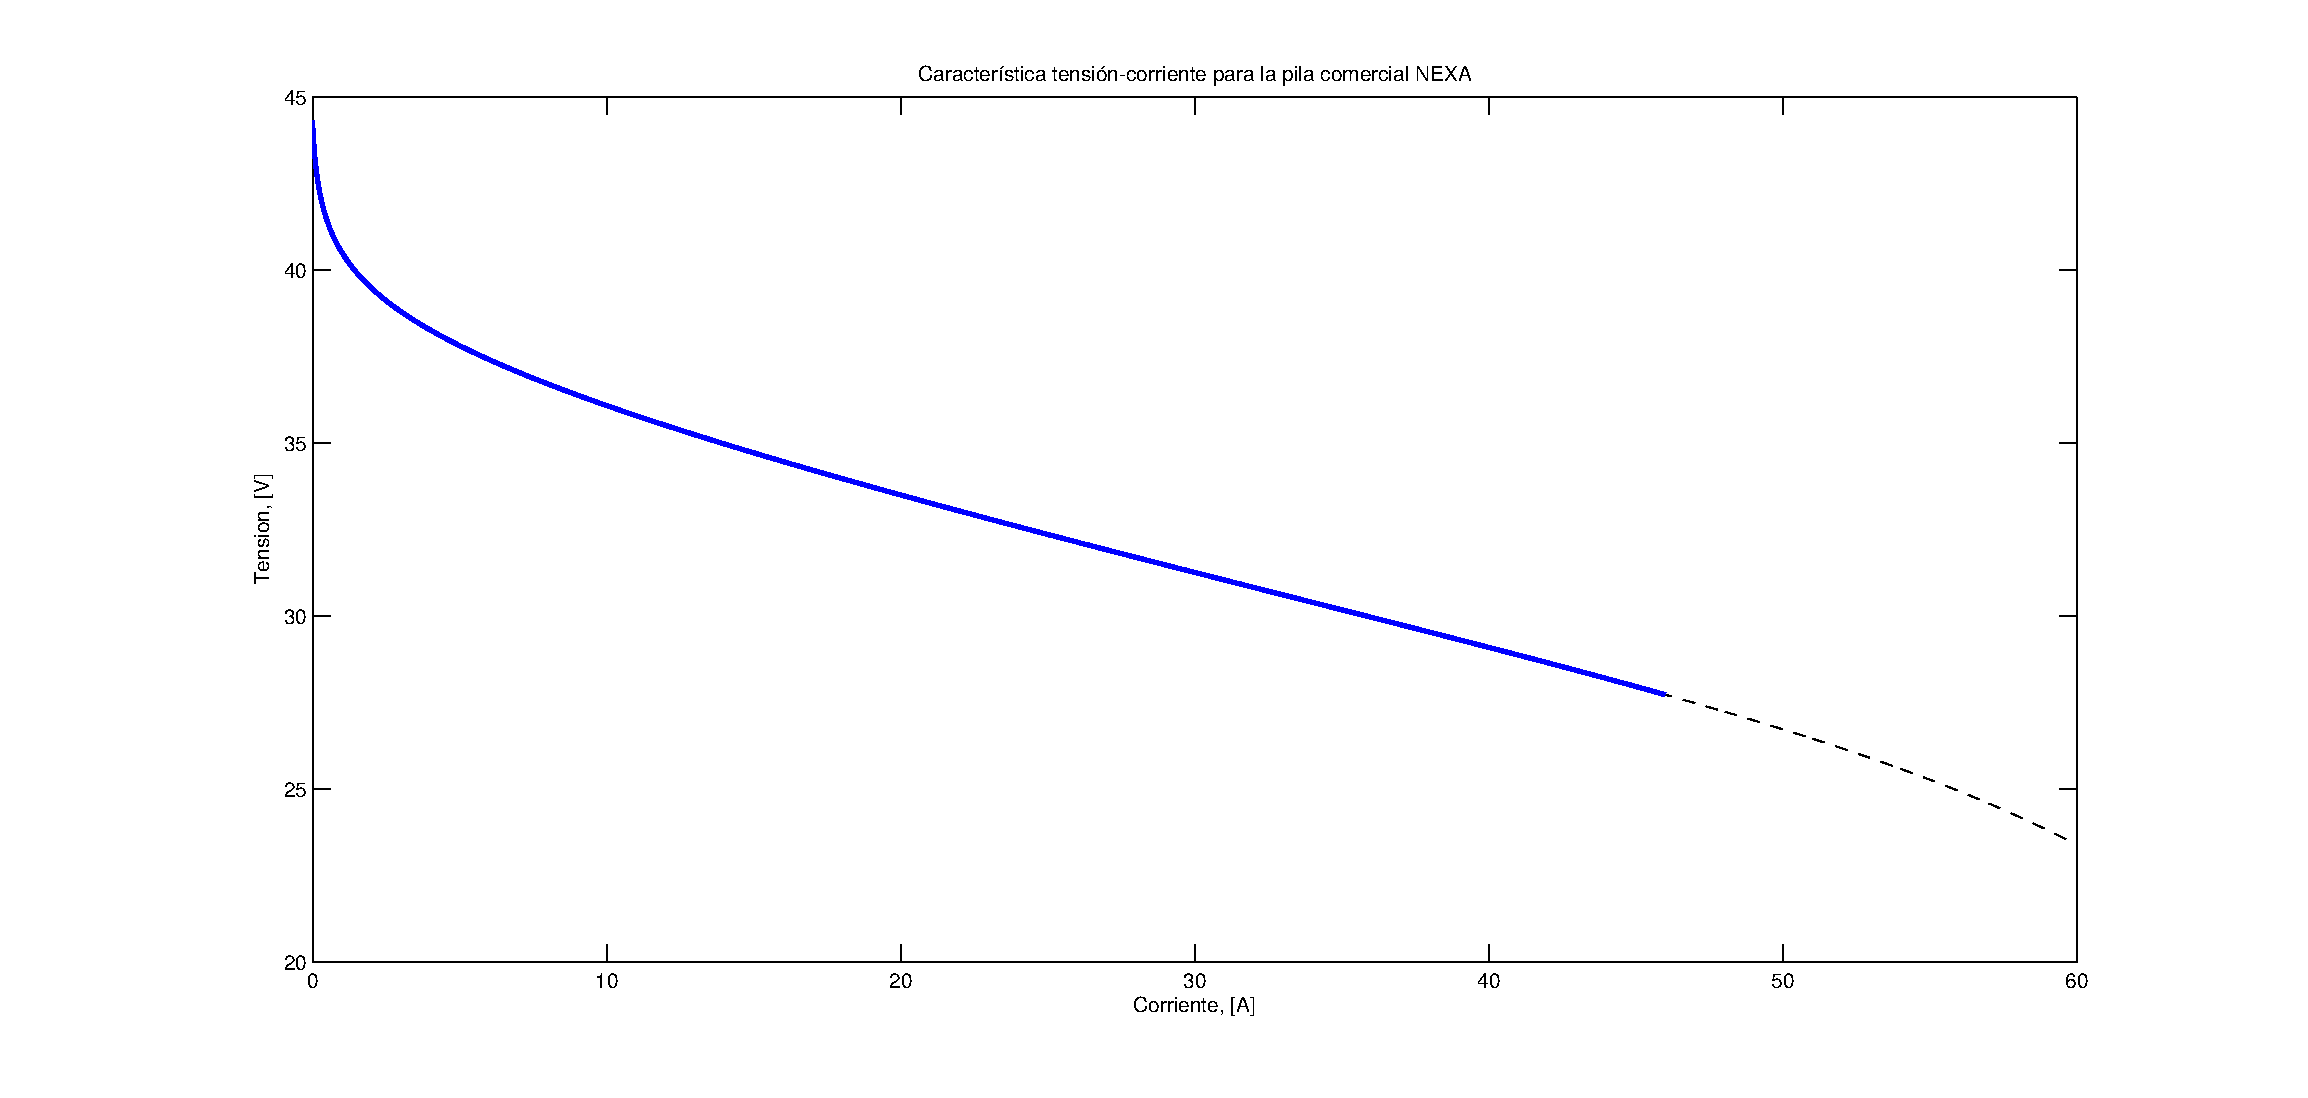
\includegraphics[width=11cm]{gfx/caracteristica_NEXA.eps}
 \caption{Característica eléctrica del módulo NEXA mostrando rango de funcionamiento.}
 \label{fig:caracteristica_NEXA}
\end{figure}

El rango de funcionamiento es bastante amplio y considerando las cargas disponibles y las limitaciones eléctricas de los convertidores de
potencia ensayados, para evaluar el correcto funcionamiento en todas las regiones de la pila se ha ajustado el área efectiva contrayendo
así la curva en el eje de corriente.

El modelo fijo sirvió para comprobar la funcionalidad del emulador ante algoritmos de un modelo más sencillo, lo cual respaldaría el
funcionamiento de otro modelo más complejo.

\subsection{Modelo paramétrico}
Con el fin de obtener un modelo con mayor flexibilidad y para posibilitar la continuidad del trabajo a un emulador más sofisticado, que
tuviese en cuenta tanto la dinámica de la pila como los elementos auxiliares del sistema completo se decidió realizar un segundo modelo
que permitiera ajustar algunos parámetros del modelo de tensión de la pila de celdas de combustible.

Los términos de (\ref{eq:tension_general}) que caracterizan las pérdidas de este modelo varían un poco respecto al utilizado
anteriormente, aunque el comportamiento cualitativo que se obtiene sigue la misma tendencia. 

La tensión $E$ mantiene la forma de (\ref{eq:tension_circuito_abierto}). Por otro lado para las pérdidas por activación se usa una
aproximación a una función exponencial de la forma $A+B(1-e^{k\cdot i})$. Las pérdidas por concentración se modelan por una expresión
de la forma $i \left( a \frac{i}{i_0} \right)^b$. En conjunto la expresión general es la siguiente:

\begin{equation}
 U_{fc}=E-[u_{o}+u_{a}(1-e^{-c_{1}i})]-[iR_{ohm}]-[i(c_{2}\frac{i}{i_{max}})^{c_{3}}
 \label{eq:tension_modelo_parametrico}
\end{equation}

La (\ref{eq:tension_modelo_parametrico}) difiere del modelo fijo especialmente en el modo que manifiestan su efecto, las caídas de tensión
debidas a los efectos de activación y concentración aunque cualitativamente la curva se presenta del mismo modo.

En el cuadro \ref{tab:parametros_modelo_2} se listan las expresiones correspondientes a los diferentes parámetros que se encuentran en 
(\ref{eq:tension_modelo_parametrico}) en el que aparecen las siguientes variables:
\begin{itemize}
 \item $T_{fc}$: la temperatura de la celda.
 \item $p_{O_2}$: la presión que ejerce el oxígeno sobre la superficie del cátodo.
 \item $p_{H_2}$: la presión del hidrógeno sobre el la superficie del ánodo.
 \item $p_{sat}$: representa la presión de saturación de vapor a una dada temperatura. La expresión que devuelve éste valor es:
 $$ p_{sat}=1,456 \times 10^-7 e^{0,04203T_{fc}} $$
\end{itemize}


\begin{table}
\centering%
\begin{tabular}{|c|p{10cm}|}
\hline 
Var. 	& \tabularnewline
\hline \hline 
$E$ 		& $1,4824-8,5\times 10^{-4}+4,308\times 10^{-5}T_{fc}(\ln(p_{H_{2}})+\frac{1}{2}\ln(p_{O_{2}}))$\tabularnewline
\hline 
$u_{0}$ 	& $0,5324-8,5\times 10^{-4}$\tabularnewline
\hline 
$u_{a}$ 	& $(-1,618\times10^{-5}T_{fc}+1,618\times10^{-2})(\frac{p_{O_{2}}}{0,1173}+p_{sat})^{2}
+(1,8\times10^{-4}T_{fc}-0,166)(\frac{p_{O_{2}}}{0,1173}+p_{sat})+(-5,8\times10^{-4}T_{fc}+0,5736)$\tabularnewline
\hline 
$c_{1}$ 	& $10$\tabularnewline
\hline 
$R_{ohm}$ 	& $0,18199e^{350(\frac{1}{T_{fc}}-\frac{1}{303})}$\tabularnewline
\hline 
$c_{2}$ 	& $(8,66\times10^{-5}T_{fc}-0,068)(\frac{p_{O_{2}}}{0,1173}+p_{sat})
+(-1,6\times10^{-4}T_{fc}+0,54)\quad para\,(\frac{p_{O_{2}}}{0,1173}+p_{sat})\geq2\, atm$\tabularnewline
\hline 
$i_{max}$ 	& $2,2$\tabularnewline
\hline 
$c_{3}$ 	& $2$\tabularnewline
\hline 
\end{tabular}\caption{Expresiones del modelo paramétrico}
\label{tab:parametros_modelo_2}
\end{table}

Para poder utilizar el modelo presentado algunas entradas han sido relacionadas ya que no se disponen del modelo dinámico
de los dispositivos auxiliares que se encargarían de ello. Las consideraciones realizadas son las siguientes:

\begin{itemize}
 \item La membrana se encuentra completamente humidificada que es el caso más favorable.
 \item La presión del cátodo y del ánodo son iguales. Normalmente se mide la presión en el cátodo
 y se regula la válvula del tanque de combustible mediante alguna acción de control de modo que 
 se iguale la presión en el ánodo.
 \item La humedad relativa de los reactivos se considera igual y fija para ambos electrodos, cercana a la presión de saturación.
\end{itemize}

La humedad relativa se define como $\Phi = \frac{p_{v}}{p_{sat}}$, donde $p_{v}$ es la presión de vapor y $p_{sat}$ es la presión de saturación.
Para el modelo presente, este parámetro ha sido fijado en $0,9$ que es un valor razonable, considerando que permite a la membrana tener un nivel
de humedad adecuado y evita que se deposite agua líquida en los colectores de los electrodos. La variable a la que se tiene acceso es entonces
la presión de cátodo, que es la misma que del ánodo.

En la fig. \ref{fig:modelo_2} se muestra un esquema del modelo con sus diferentes entradas con valores definidos para cada variable. 
La fig. \ref{fig:curvas_modelo_2} muestra una serie de curvas de la tensión devuelta por la pila a diferentes temperaturas y presiones.

\begin{figure}[H]
 \centering
 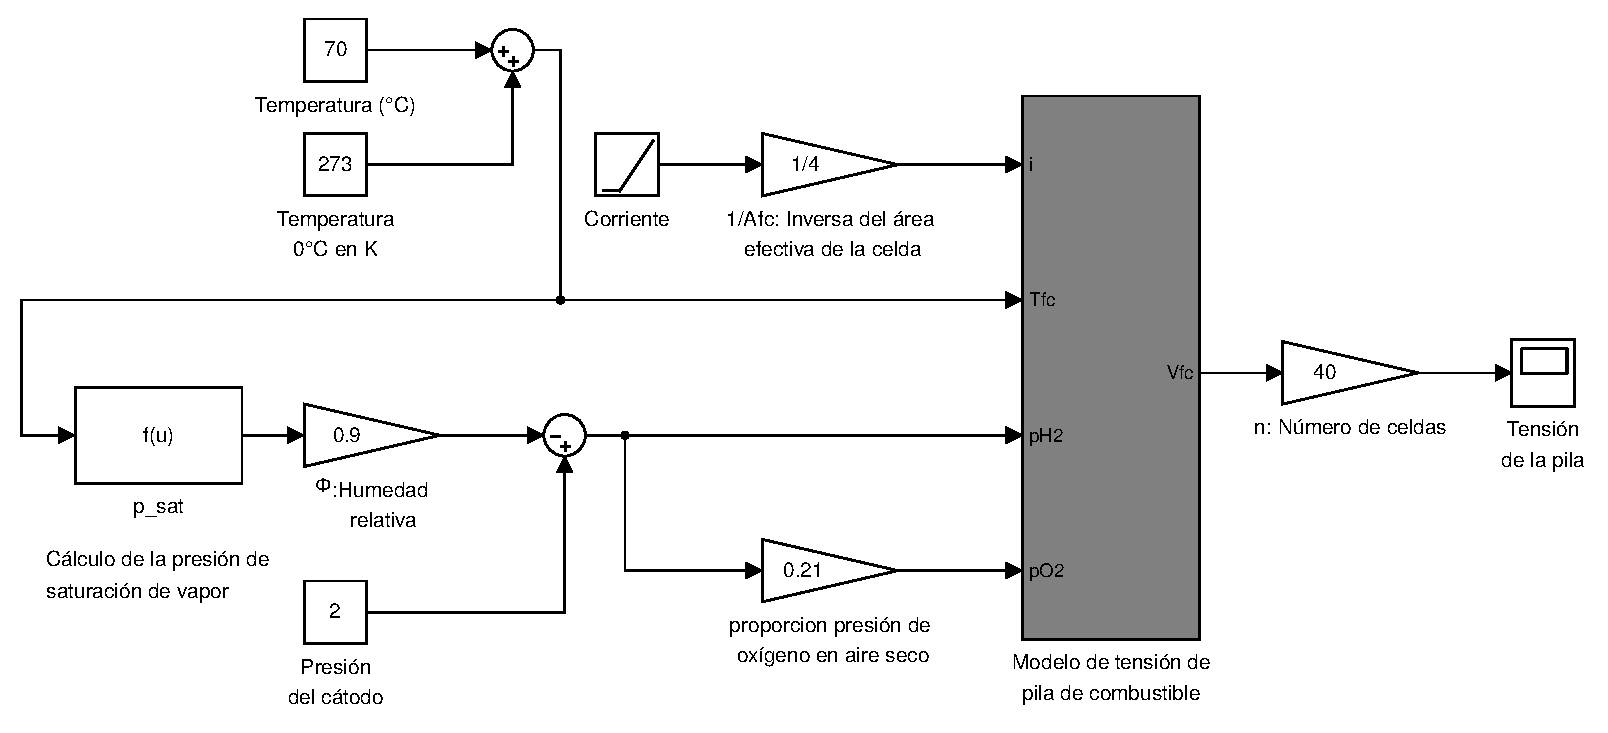
\includegraphics[width=11cm]{gfx/modelo_2.eps}
 \caption{Diagrama esquemático del modelo de tensión de la celda parametrizado}
 \label{fig:modelo_2}
\end{figure}

\begin{figure}
 \centering
 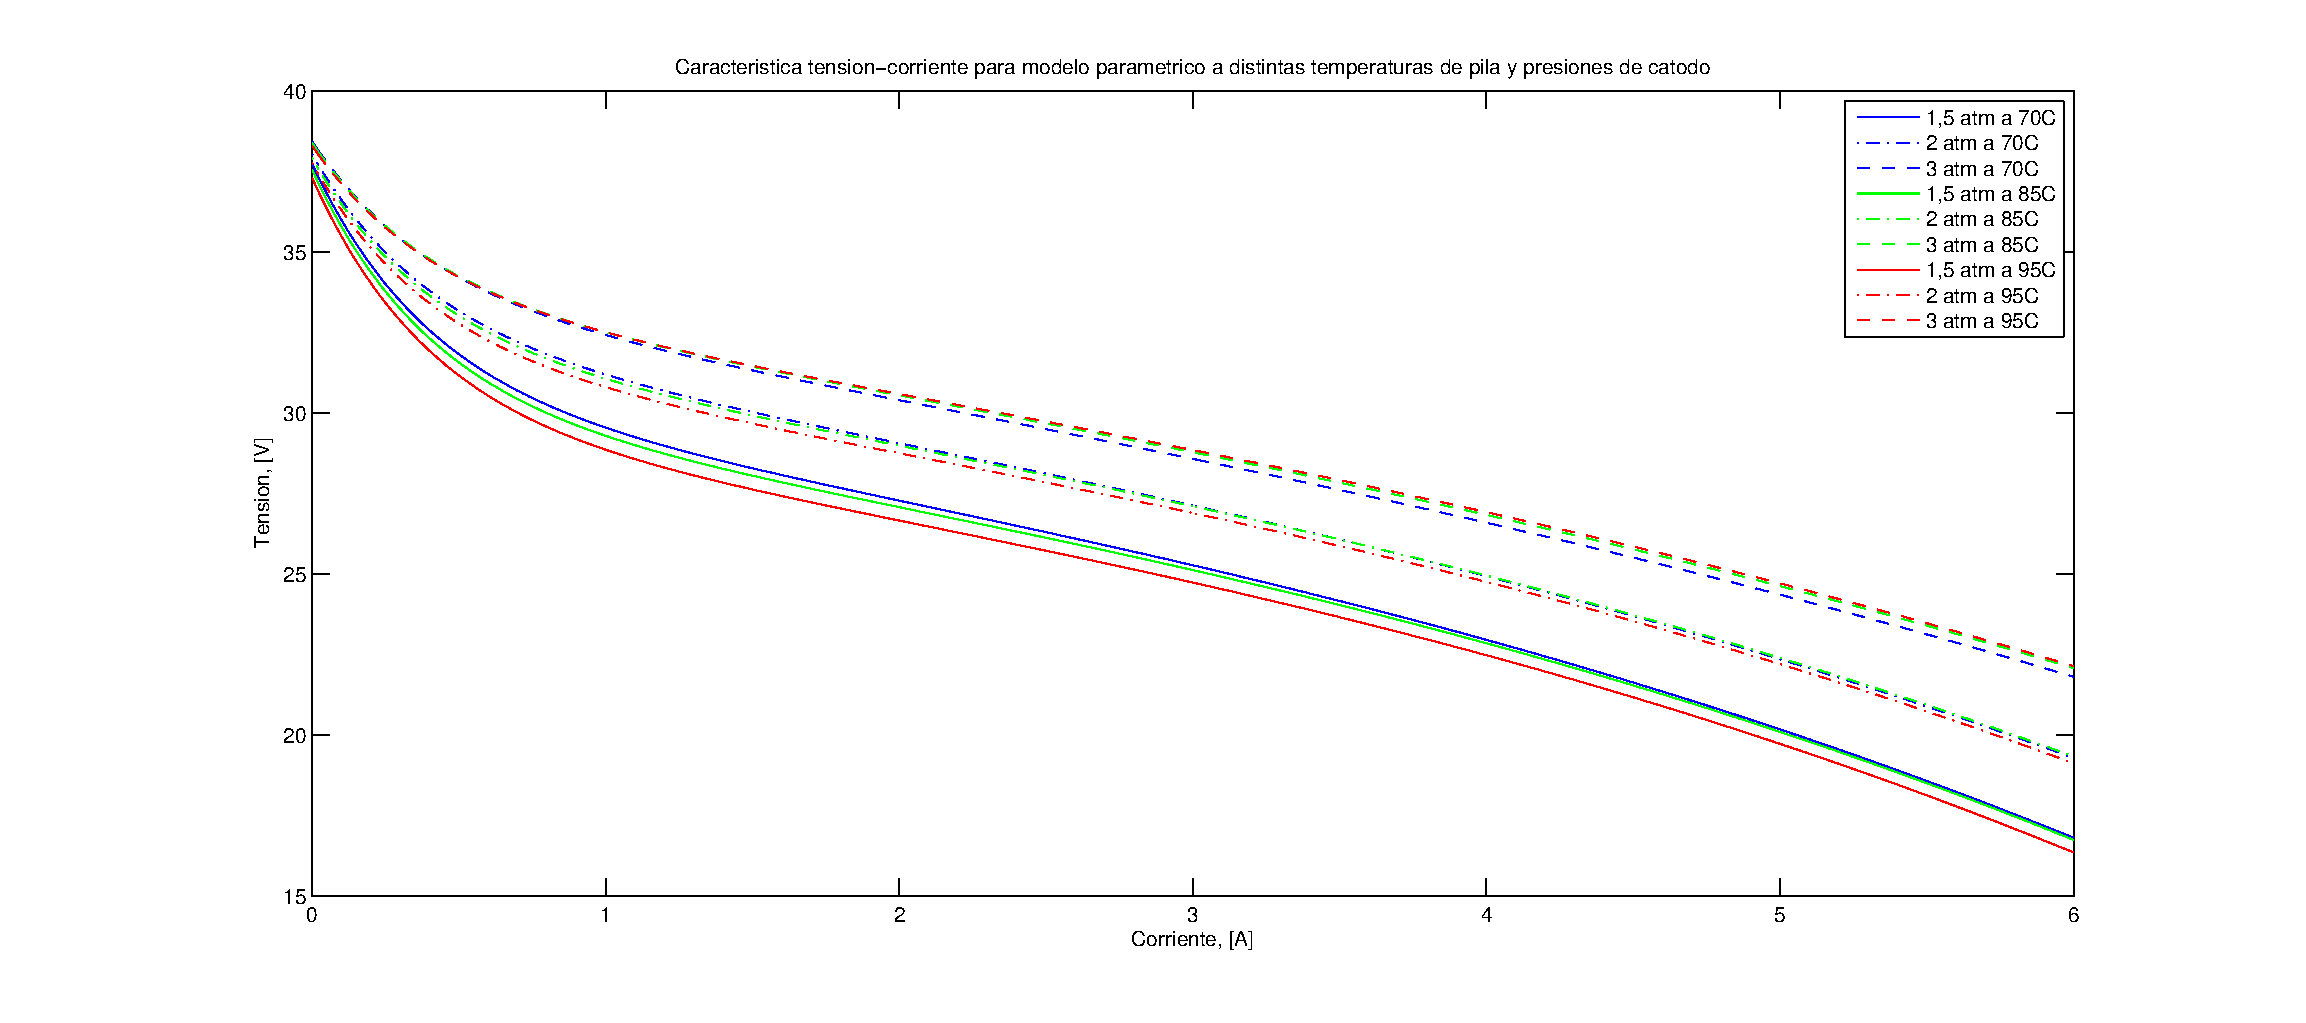
\includegraphics[width=11cm]{gfx/I-V.eps}
 \caption{Diagrama esquemático del modelo de tensión de la celda parametrizado}
 \label{fig:curvas_modelo_2}
\end{figure}

\section{Comentarios}
Con los modelos presentados y los fundamentos teóricos que los avalan se puede proceder a su implementación práctica.
Hará falta un soporte físico para ello, el cual consta de un \emph{convertidor conmutado}. Estos convertidores poseen características
que los hacen muy apropiados para este trabajo, especialmente por su eficiencia frente a otras opciones. Y el atributo que permitirá que este
dispositivo sea capaz de emular el correcto comportamiento de las FC's residen en el mecanismo de control que se establece a través de modulación
de ancho de pulso. Esto ofrece gran flexibilidad al momento de realizar cambios en el comportamiento general del convertidor y es lo que se busca
para introducir los modelos estudiados en el presente capitulo.
\end{comment}
